\documentclass[../entwurf.tex]{subfiles}
\begin{document}

	\section{Model}
		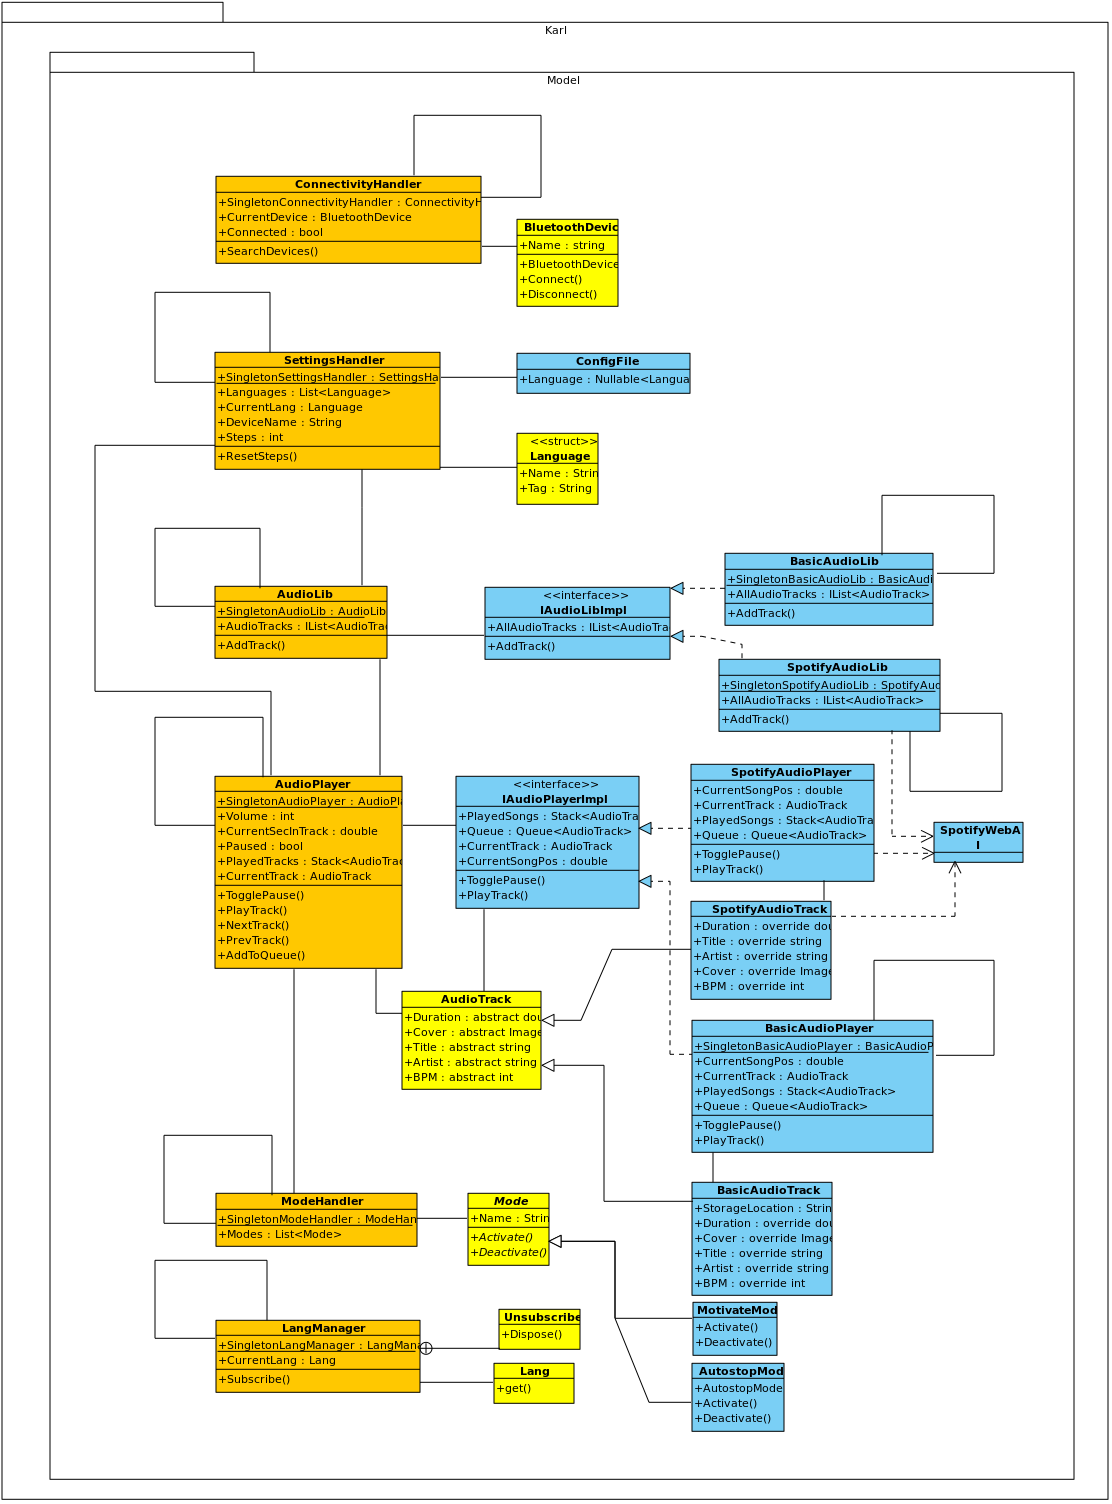
\includegraphics[width=\textwidth,height=\textheight,keepaspectratio]{../graphics/uml_diagramme/Model.png}
		\newpage
		Im UML Diagramm sind hier die Orangenen Klassen, die Schnittstellenklassen, also Fassaden zum einfachen 
		Zugriff auf bestimmte zusammenhängende Teile des Models. Auch die gelb eingefärbten Klassen sind Klassen zur 
		u.A. externen Kommunikation. Die Blau eingefärbten Klassen arbeiten im Hintergrund.
		\subsection{Schnittstelle}
			Die Schnittstelle zu den ViewModels besteht aus Klassen, die explizit konzipiert sind um die Kommunikation zwischen ViewModels und Model
			einfach zu gestalten. Alle Klassen der Schittstelle sind nach dem 
			Singleton-Muster\footnote{\see[Muster 2: ]{https://csharpindepth.com/Articles/Singleton}} aufgebaut.
			\subsubsection{ConnectivityHandler}
				\sign{public class ConnectivityHandler}
				Diese Klasse sucht nach Bluetooth Geräten, mit denen man sich verbinden kann.
				\paragraph{Attribute:}
					\begin{itemize}
						\i{private IEarable Earable} Die Schnittstelle zur EarablesLibrary.
					\end{itemize}
				\paragraph{Properties:}
					\begin{itemize}
						\i{public BluetoothDevice CurrentDevice} Das aktuell verbundene eSense Gerät. Definiert keinen Setter, da dieses nur vom Model
						verwaltet werden soll.
						\i{public bool Connected} Boolscher Wert, ob earables verbunden sind. Definiert keinen Setter.
					\end{itemize}
				\paragraph{Methoden:}
					\begin{itemize}
						\i{public ObservableCollection<BluetoothDevice> SearchDevices()} Sucht nach Bluetooth Geräten in der Nähe.
					\end{itemize}
			\subsubsection{AudioLib}
				\sign{class AudioLib}
				Die Fassade für den einfachen Zugriff auf das aktuelle Audiomodul.
				\paragraph{Attribute:}
					\begin{itemize}
						\i{private AudioLib \_singletonAudioLib} Dies ist das singleton Attribut.
						\i{private IAudioLibImpl AudioLibImp} Dies ist die konkrete Implementierung der
						AudioLib
					\end{itemize}
				\paragraph{Properties:}
					\begin{itemize}
						\i{public AudioLib SingletonAudioLib} Dies ist die Property die ein Getter für den
						Singleton definiert. Daher gibt es kein Setter.
						\i{public AudioTrack CurrentTrack} Dies ist das momentan ausgewählte Lied. Dieses
						wird auch im AudioPlayer abgepielt und angezeigt.
						\i{public IList<AudioTrack> AudioTracks} Dies ist eine Liste aller Tracks in dieser
						Bibliothek. Es gibt keinen Setter da diese von der konkreten Bibliothek verwaltet werden soll.
					\end{itemize}
				\paragraph{Methoden:}
					\begin{itemize}
						\i{public void AddTrack(String Indentifier, String Name, String Artist, int BPM)} 
						Dies fügt der aktuellen konkreten Bibliothek ein neuen Track hinzu,
						falls diese das unterstützt.
						\i{public void NextSong()} Dies überspringt den aktuellen Song und spielt einen neuen Song ab.
						Der aktuelle als erstes Element von PlayedTracks eingefügt.
						\i{public void PrevSong()} Dies ruft \textit{CurrentTrack = AudioLibImpl.PlayedTracks.Pop()} auf.
					\end{itemize}
			\subsubsection{AudioPlayer}
				\sign{class AudioPlayer}
				Diese Klasse ist eine Fassade zum einfachen Zugriff auf den aktuellen konkreten AudioPlayer.
				\paragraph{Attribute:}
					\begin{itemize}
						\i{private AudioLib AudioLib} Dies ist das Singleton Objekt von AudioLib zum einfachen Zugriff.
					\end{itemize}
				\paragraph{Properties:}
					\begin{itemize}
						\i{public int Volume} Hier wird eine Getter und Setter für die Systemlautstärke definiert.
						\i{public double CurrentSecInTrack} Hier werden Getter und Setter für die Position im Song definiert.
						\i{public bool Paused} Hier werden Getter und Setter für den Wahrheitswert, ob das Lied pausiert ist definiert.
					\end{itemize}
				\paragraph{Methoden:}
					\begin{itemize}
						\i{public void TogglePause()} Diese Methode negiert den Boolean Paused.
						\i{public void PlayTrack()} Diese Methode startet den Playback des CurrentSong der AudioLib
						\i{public void NextTrack()} Diese Methode ruft AudioLib.NextTrack() und PlayTrack() auf.
						\i{public void PrevTrack()} Diese Methode ruft AudioLib.PrevTrack() und PlayTrack() auf.
					\end{itemize}
			\subsubsection{SettingsHandler}
				\sign{public class SettingsHandler}
				Diese Klasse ist die Fassade zum Zugriff auf die App-Einstellungen. Sie verwendet dafür die Klasse ConfigFile.
				\paragraph{Attribute:}
					\begin{itemize}
						\i{private ConfigFile ConfigFile} Das Objekt der Klasse Config-File.
					\end{itemize}
				\paragraph{Properties:}
					\begin{itemize}
						\i{public List<Language> Languages} Die Liste aller registrierten Sprach-Dokumente. Definiert keinen Setter.
						\i{public Language CurrentLang} Die aktuell ausgewählte Sprache.
						\i{public String DeviceName} Der Name des verbundenen Bluetooth Gerät.
						\i{public int Steps} Die in allen Sessions seit dem letzten reset gelaufenen Schritte. Definiert keinen Setter.
					\end{itemize}
				\paragraph{Methoden:}
					\begin{itemize}
						\i{public void ResetSteps()} Diese Metjode setzt die Anzahl der gezählten Schritte zurück.
					\end{itemize}
			\subsubsection{ModeHandler}
				\sign{public class ModeHandler}
				Diese Klasse ist verwaltet die aktivierten und deaktivierten Modi.
				\paragraph{Properties:}
					\begin{itemize}
						\i{public List<Mode> Modes} Dies ist die Liste aller beim ModeHandler registrierten Modi.
					\end{itemize}
		\subsection{Audio Modul}
			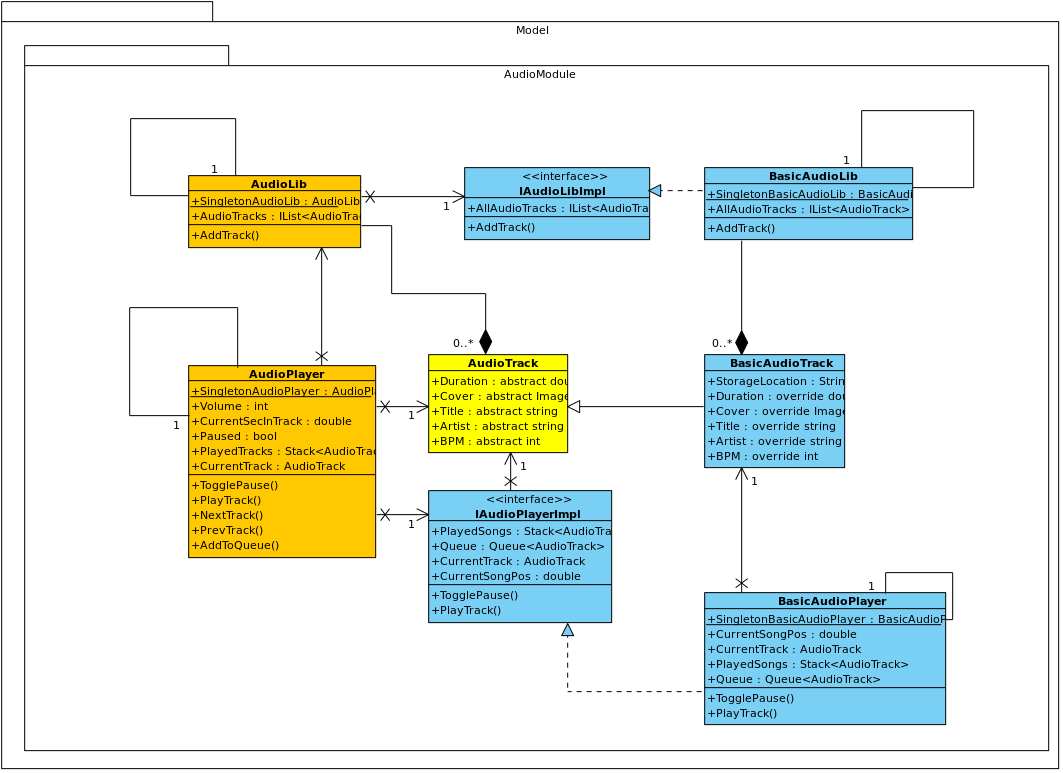
\includegraphics[scale=0.3]{../graphics/uml_diagramme/AudioModule.png}\\
			Das Audio-Modul besteht jeweils aus der Audiobibliothek und dem Audioplayer.
			Bei beiden wird zwischen der Fassade (in der Schnittstelle) und der Implementierung (hier) unterschieden.
			Dadurch werden Konsistenzprobleme vermieden, da nicht unterschiedliche Teile der App auf unterschiedliche konkrete Implementierungen
			zugreifen können. Bzw. immer wissen, was die aktuelle Implementierung ist.
			Zusätzlich gibt es noch die Klasse AudioTrack welche einen konkreten AudioTrack zu einer konkreten Implementierung definiert.
			\subsubsection{IAudioLibImpl}
				\sign{interface IAudioLibImpl}
				Dieses Interface stellt eine konkrete Implementierung einer Audio Bibliothek dar.
				\paragraph{Properties:}
					\begin{itemize}
						\i{Stack<AudioTrack> PlayedSongs} Dies ist der Stack der schon gespielten Lieder der Implementierung.
						Das erste Listenelement ist der zuletzt abgespielte Track. Es gibt keinen Setter.
						\i{AudioTrack CurrentTrack} Dies ist der konkrete aktuelle Song.
						\i{IList<AudioTrack> AllAudioTracks} Das ist die konkrete Liste aller Songs in dieser Audio Bibliothek.
					\end{itemize}
				\paragraph{Methoden:}
					\begin{itemize}
						\i{void AddTrack()} Dies fügt der konkreten Implementierung der Audio Bibliothek einen neuen Track hinzu, sofern
						diese das unterstützt.
					\end{itemize}
			\subsubsection{IAudioPlayerImpl}
				\sign{interface IAudioPlayerImpl}
				Dieses Interface stellt eine konkrete Implementierung des Audio Players dar.
				\paragraph{Properties:}
					\begin{itemize}
						\i{double CurrentSongPos} Dies definiert Getter und Setter für die aktuelle Position im Lied.
					\end{itemize}
				\paragraph{Methoden:}
					\begin{itemize}
						\i{void TogglePause()} Dies Pausiert den Song/Spielt den Song weiter ab.
						\i{void PlayTrack()} Dies Spielt den aktuell gewählten Song ab.
					\end{itemize}
			\subsubsection{AudioTrack}
				\sign{abstract class AudioTrack}
				Diese Klasse definiert einen Abstrakten AudioTrack.
				\paragraph{Properties:}
					Keine der Properties definiert eine set() Methode, da manche AudioLib-Implementierungen (z.B. Spotify) so etwas nicht
					unterstützen. Neben BPM kann die Schnittstelle für weitere Eigenschaften des Songs erweitert werden.
					\begin{itemize}
						\i{public abstract double Duration} Die Dauer des Tracks.
						\i{public abstract Image Cover} Das Bild welches dem Song zugewiesen ist. Image ist eine Xamarin.Forms Klasse.
						\i{public abstract string Title} Der Name des Songs.
						\i{public abstract string Artist} Der Name des Künstlers.
						\i{public abstract int BPM} Der BPM Wert der diesem Song hinterlegt ist.
					\end{itemize}
			\subsubsection{BasicAudioLib}
				\sign{sealed class BasicAudioLib : IAudioLibImpl}
				Diese Klasse definiert eine Standart Audio Bibliothek. Sie speichert den Ort der Audio Datei und andere Eigenschaften hinterlegter
				Songs. Sie ist nach dem Singleton Muster aufgebaut und hat die dazugehörigen Properties und Attribute.
			\subsubsection{BasicAudioPlayer}
				\sign{sealed class BasicAudioPlayer : IAudioPlayerImpl}
				Diese Klasse definiert einen simplen Audio Player, welcher Audio Dateien aus dem internen Speicher auslesen und abspielen kann.
			\subsubsection{BasicAudioTrack}
				\sign{sealed class BasicAudioTrack : AudioTrack}
				Diese Klasse definiert einen AudioTrack zum BasicAudioPlayer und zur BasicAudioLib.
				\paragraph{Attribute:}
					\begin{itemize}
						\i{public String StorageLocation} Dieser String stellt dar, wo im Speicher die zugrundeliegende Audio-Datei liegt.
					\end{itemize}
			\subsubsection{SpotifyAudioLib}
				\sign{sealed class SpotifyAudioLib : IAudioLibImpl}
				Diese Klasse implementiert eine konkrete Audio Bibliothek mit Spotify Integration.
				Sie hat als Grundlage eine Spotify Playlist. Sie kommuniziert mit der Klasse SpotifyWebAPI.
				Sie ist nach dem Singleton Muster aufgebaut und hat die dazugehörigen Properties und Attribute.
				\paragraph{Attribute:}
					\begin{itemize}
						\i{private String PlaylistTag} Dieser String repräsentiert den Tag der gewählten Spotify Playlist.
					\end{itemize}
			\subsubsection{SpotifyAudioPlayer}
				\sign{sealed class SpotifyAudioPlayer : IAudioPlayerImpl}
				Dies ist die Implementierung des Audio Player für Spotify. Die Klasse kommuniziert mit der Klasse SpotifyWebAPI.
			\subsubsection{SpotifyAudioTrack}
				\sign{sealed class SpotifyAudioTrack : AudioTrack}
				Diese Klasse definiert einen AudioTrack zum SpotifyAudioPlayer und zur SpotifyAudioLib.
				\paragraph{Attribute:}
					\begin{itemize}
						\i{private String Tag} Dies repräsentiert den Tag des Spotify Track.
					\end{itemize}
			\subsubsection{SpotifyWebAPI}
				\sign{sealed class SpotifyWebAPI}
				Diese Klasse dient zur Kommunikation mit der Spotify-Web-API. Sie wird die Library 
				SpotifyAPI-NET\footnote{\see[]{https://github.com/JohnnyCrazy/SpotifyAPI-NET}} verwenden.
				Sie ist nach dem Singleton Muster aufgebaut und hat die dazugehörigen Properties und Attribute.
		\subsection{Modi}
			Dies sind die verschiedenen Modi, welche aktiv oder inaktiv sein können.
			\subsubsection{Mode}
				\sign{public abstract class Mode}
				Die abstrakte Klasse Mode definiert einen Generellen Modus und bietet eine Schnittstelle zu den ViewModels.
				\paragraph{Properties:}
					\begin{itemize}
						\i{public String Name} Dies ist der Name des konkreten Modus.
					\end{itemize}
				\paragraph{Methoden:}
					\begin{itemize}
						\i{protected Mode()} Da die Klasse abstrakt ist, ist der Konstruktor protected. Er updated den Namen des Modus.
						\i{public abstract void Activate()} Diese Methode aktiviert diesen Modus.
						\i{public abstract void Deactivate()} Diese Methode deaktiviert diesen Modus.
						\i{protected abstract String UpdateName(Lang value)}  Diese Methode liefert den Namen des Modus zurück. Der Parameter das
						Objekt aus dem die konkrete Klasse ihren Namen beziehen kann.
					\end{itemize}
			\subsubsection{AutostopMode}
				\sign{class AutostopMode : Mode}
				Der konkrete Autostop-Modus.
			\subsubsection{MotivateMode}
				\sign{class MotivateMode : Mode}
				Der konkrete Motivationsmusik-Modus.
		\subsection{Einstellungen}
			Hier sind die Klassen bezüglich der App-Einstellungen und Sprach-Einstellungen.
			\subsubsection{ConfigFile}
				\sign{class ConfigFile}
				Die Klasse ConfigFile liest, schreibt und verwaltet das .config Dokument im Speicher der App.
				\paragraph{Properties:}
					\begin{itemize}
						\i{public Nullable<Language> Language} Die verwendete Sprache. Nullable, falls die Sprache nicht gelesen werden kann.
						\i{String AudioModule} Der Indentifier des aktuell verwendeten Audio Moduls.
						\i{int TotalSteps} Die Anzahl aller Schritte seit letztem Reset.
					\end{itemize}
			\subsubsection{LangManager}
				\sign{public class LangManager : IObservable<Lang>}
				Der LangManager ist ein Observable nach dem 
				C\# Observable Pattern\footnote{\see[]{https://docs.microsoft.com/en-us/dotnet/api/system.iobservable-1?view=netframework-4.8}}
				Er lädt alle verfügbaren Sprachen aus dem internen Speicher aus .lang Text-Dokumenten.
				Die Klasse ist implementiert ein Singleton-Muster.
				\paragraph{Properties:}
					\begin{itemize}
						\i{public Lang CurrentLang} Die aktuell gewählte Sprache.
					\end{itemize}
			\subsubsection{Lang}
				\sign{public class Lang}
				Die Klasse Lang definiert genau eine Sprache und alle zugehörigen Strings. 
				\paragraph{Methoden:}
					\begin{itemize}
						\i{public String get(String tag)} Der Rückgabe-String ist genau der String der mit dem Parameter-String assoziiert wird.
					\end{itemize}
			\subsubsection{Language}
				\sign{struct Language}
				\paragraph{Properties:}
					\begin{itemize}
						\i{public String Name} Der Name der Sprache.
						\i{public String Tag} Der Tag der Sprache um das Dokument zu identifizieren.
					\end{itemize}
		\subsection{Sonstige}
			\subsubsection{BluetoothDevice}
				\sign{public class BluetoothDevice}
				Ein Adapter zwischen IEarable der EarableLibrary und dem ViewModel.
				\paragraph{Attribute:}
					\begin{itemize}
						\i{private IEarable \_earable} Das zugrundeliegende IEarable Objekt.
					\end{itemize}
				\paragraph{Properties:}
					\begin{itemize}
						\i{public string Name} Der Bluetooth-Name des Geräts.
					\end{itemize}
				\paragraph{Methoden:}
					\begin{itemize}
						\i{public void Connect()} Bluetooth-Verbindung mit diesem Gerät herstellen.
						\i{public void Disconnect()} Bluetooth-Verbindung mit diesem Gerät trennen.
					\end{itemize}
					
\end{document}
